\documentclass{article}
\usepackage[utf8]{inputenc}
\usepackage{graphicx}
\usepackage{hyperref}
\date{\vspace{-10ex}}
\title{Task1: Creating a small image processing library}

\begin{document}

\maketitle

%\section{Accelerating Matrix Multiplication}

By: \textbf{Rachit Kumar}-2017CS10364  \href{mailto:cs1170364@iitd.ac.in}{cs1170364@iitd.ac.in}
\\
\textbf{ Rahul Choudhary}-2017CS10365 \href{mailto:cs1170365@iitd.ac.in}{cs1170365@iitd.ac.in}

\section{In this, we have implemented five main functions, namely:}

\begin{itemize}
\tightlist
\item
  Convolution(with and without input padding, as convolution and as
  matrix multiplication(multiplication implemented using mkl, openblas,
  pthreads and iterative formula))
\item
  Non-linear activations(relu and tanh)
\item
  Subsampling(maxpooling and average pooling)
\item
  Converting a vector of random floats to a vector of
  probabilities(softmax and sigmoid)
 \item 
  Implementation of LeNet architecture 
\end{itemize}

\section{Input formats:}

\begin{itemize}
\tightlist
\item \textbf{Convolution without input padding:}

./output convolution\_withoutpadding
matrix1.txt matrix1\_numrows matrix2.txt matrix2\_numrows

\item \textbf{Convolution with input padding:}

./output convolution\_withpadding padsize
matrix1.txt matrix1\_numrows matrix2.txt matrix2\_numrows


\item \textbf{Convolution without input padding as matrix multiplication:}

./output
convolution\_withoutpadding\_matrixmult matrix1.txt matrix1\_numrows
matrix2.txt matrix2\_numrows
(method of matrixmult(manual/mkl/openblas/pthread))

\item \textbf{Convolution with input padding as matrix multiplication:}

./output convolution\_withpadding\_matrixmult
padsize matrix1.txt matrix1\_numrows matrix2.txt matrix2\_numrows
 (methodof multiplication (manual/mkl/openblas/pthread))

\item \textbf{relu function on matrix elements:}

./output activation relu matrix.txt
number\_of\_rows\_in\_matrix number\_of\_columns\_in\_matrix

\item \textbf{tanh function on matrix elements:}

./output activation tanh matrix.txt
number\_of\_rows\_in\_matrix number\_of\_columns\_in\_matrix

In this function, we apply tanh function(i.e.
f(x)=(exp(x)-exp(-x))/(exp(x)+exp(-x))) on each individual element of
the given matrix.

\item \textbf{Maxpooling of square matrices:}

./output subsampling maxpooling matrix.txt
number\_of\_rows\_in\_input\_matrix
number\_of\_rows\_in\_output\_matrix


\item \textbf{Average pooling of square matrices:}

./output subsampling avgpooling matrix.txt
number\_of\_rows\_in\_input\_matrix
number\_of\_rows\_in\_output\_matrix

\item \textbf{Sigmoid:}

./output probability sigmoid vector.txt
size\_of\_vector

\item \textbf{Softmax:}

./output probability softmax vector.txt
size\_of\_vector

\item \textbf{LeNet:}

./output lenet input.txt

\end{itemize}


\section{Performance comparision:}
\begin{itemize}
\tightlist
\item
For very small inputs and kernel, the order of time taken is: OpenBLAS $>$ Iterative Multiplication $>$ pthread $>$ MKL. As we increase the matrix size, MKL starts to become faster and faster and for large inputs, they take almost the same time. 
\item
pthread is initially much slower than normal multiplication but then for large inputs, it takes time comparable to that of normal multiplication. But on much larger inputs, it again starts to take much more time than the normal multiplication. Also, the performance of pthreads depends greatly on the number of cores in the machine on which the code is used. For best performance, the number of threads in the code should be equal to the number of cores in the machine(which in our case was two).
\end{itemize}


\begin{tabular}{|c|c|}
\hline
\multicolumn{2}{|c|}{MKL}
 \\
\hline
\textbf{size}&\textbf{time(ns)}\\
\hline
16X16&9.5x10^6\\
\hline
32X32&8.5x10^6\\
\hline
64X64&9x10^6\\
\hline
128X128&1x10^7\\
\hline
256X256&1.25x10^7\\
\hline
512X512&2.5x10^7\\
\hline
1024X1024&7.5x10^7\\
\hline
\end{tabular}
\quad
\begin{tabular}{|c|c|}
\hline
\multicolumn{2}{|c|}{OpenBLAS}\\
\hline
\textbf{size}&\textbf{time(ns)}\\
\hline
16X16& very low\\
\hline
32X32&10^5\\
\hline
64X64&2.5x10^5\\
\hline
128X128&3.5x10^5\\
\hline
256X256&1.5X10^7\\
\hline
512X512&4.75x10^7\\
\hline
1024X1024&8x10^7\\
\hline
\end{tabular}
\\\\

\begin{tabular}{|c|c|}
\hline
\multicolumn{2}{|c|}{pthread}\\
\hline
\textbf{size}&\textbf{time(ns)}\\
\hline
16X16&very low\\
\hline
32X32&4x10^5\\
\hline
64X64&2x10^6\\
\hline
128X128&8x10^6\\
\hline
256X256&3x10^7\\
\hline
512X512&8x10^7\\
\hline
1024X1024&9.5x10^7\\
\hline
\end{tabular}
\quad
\begin{tabular}{|c|c|}
\hline
\multicolumn{2}{|c|}{Manual}\\
\hline
\textbf{size}&\textbf{time(ns)}\\
\hline
16X16&very low\\
\hline
32X32&2.5x10^5\\
\hline
64X64&1x10^6\\
\hline
128X128&4x10^6\\
\hline
256X256&2x10^7\\
\hline
512X512&8x10^7\\
\hline
1024X1024&3x10^8\\
\hline
\end{tabular}
\\\\

%\graphicspath{ {/MacintoshHD/Users/eric_the_red/Desktop/cop290/ass3/PLOTS/} }

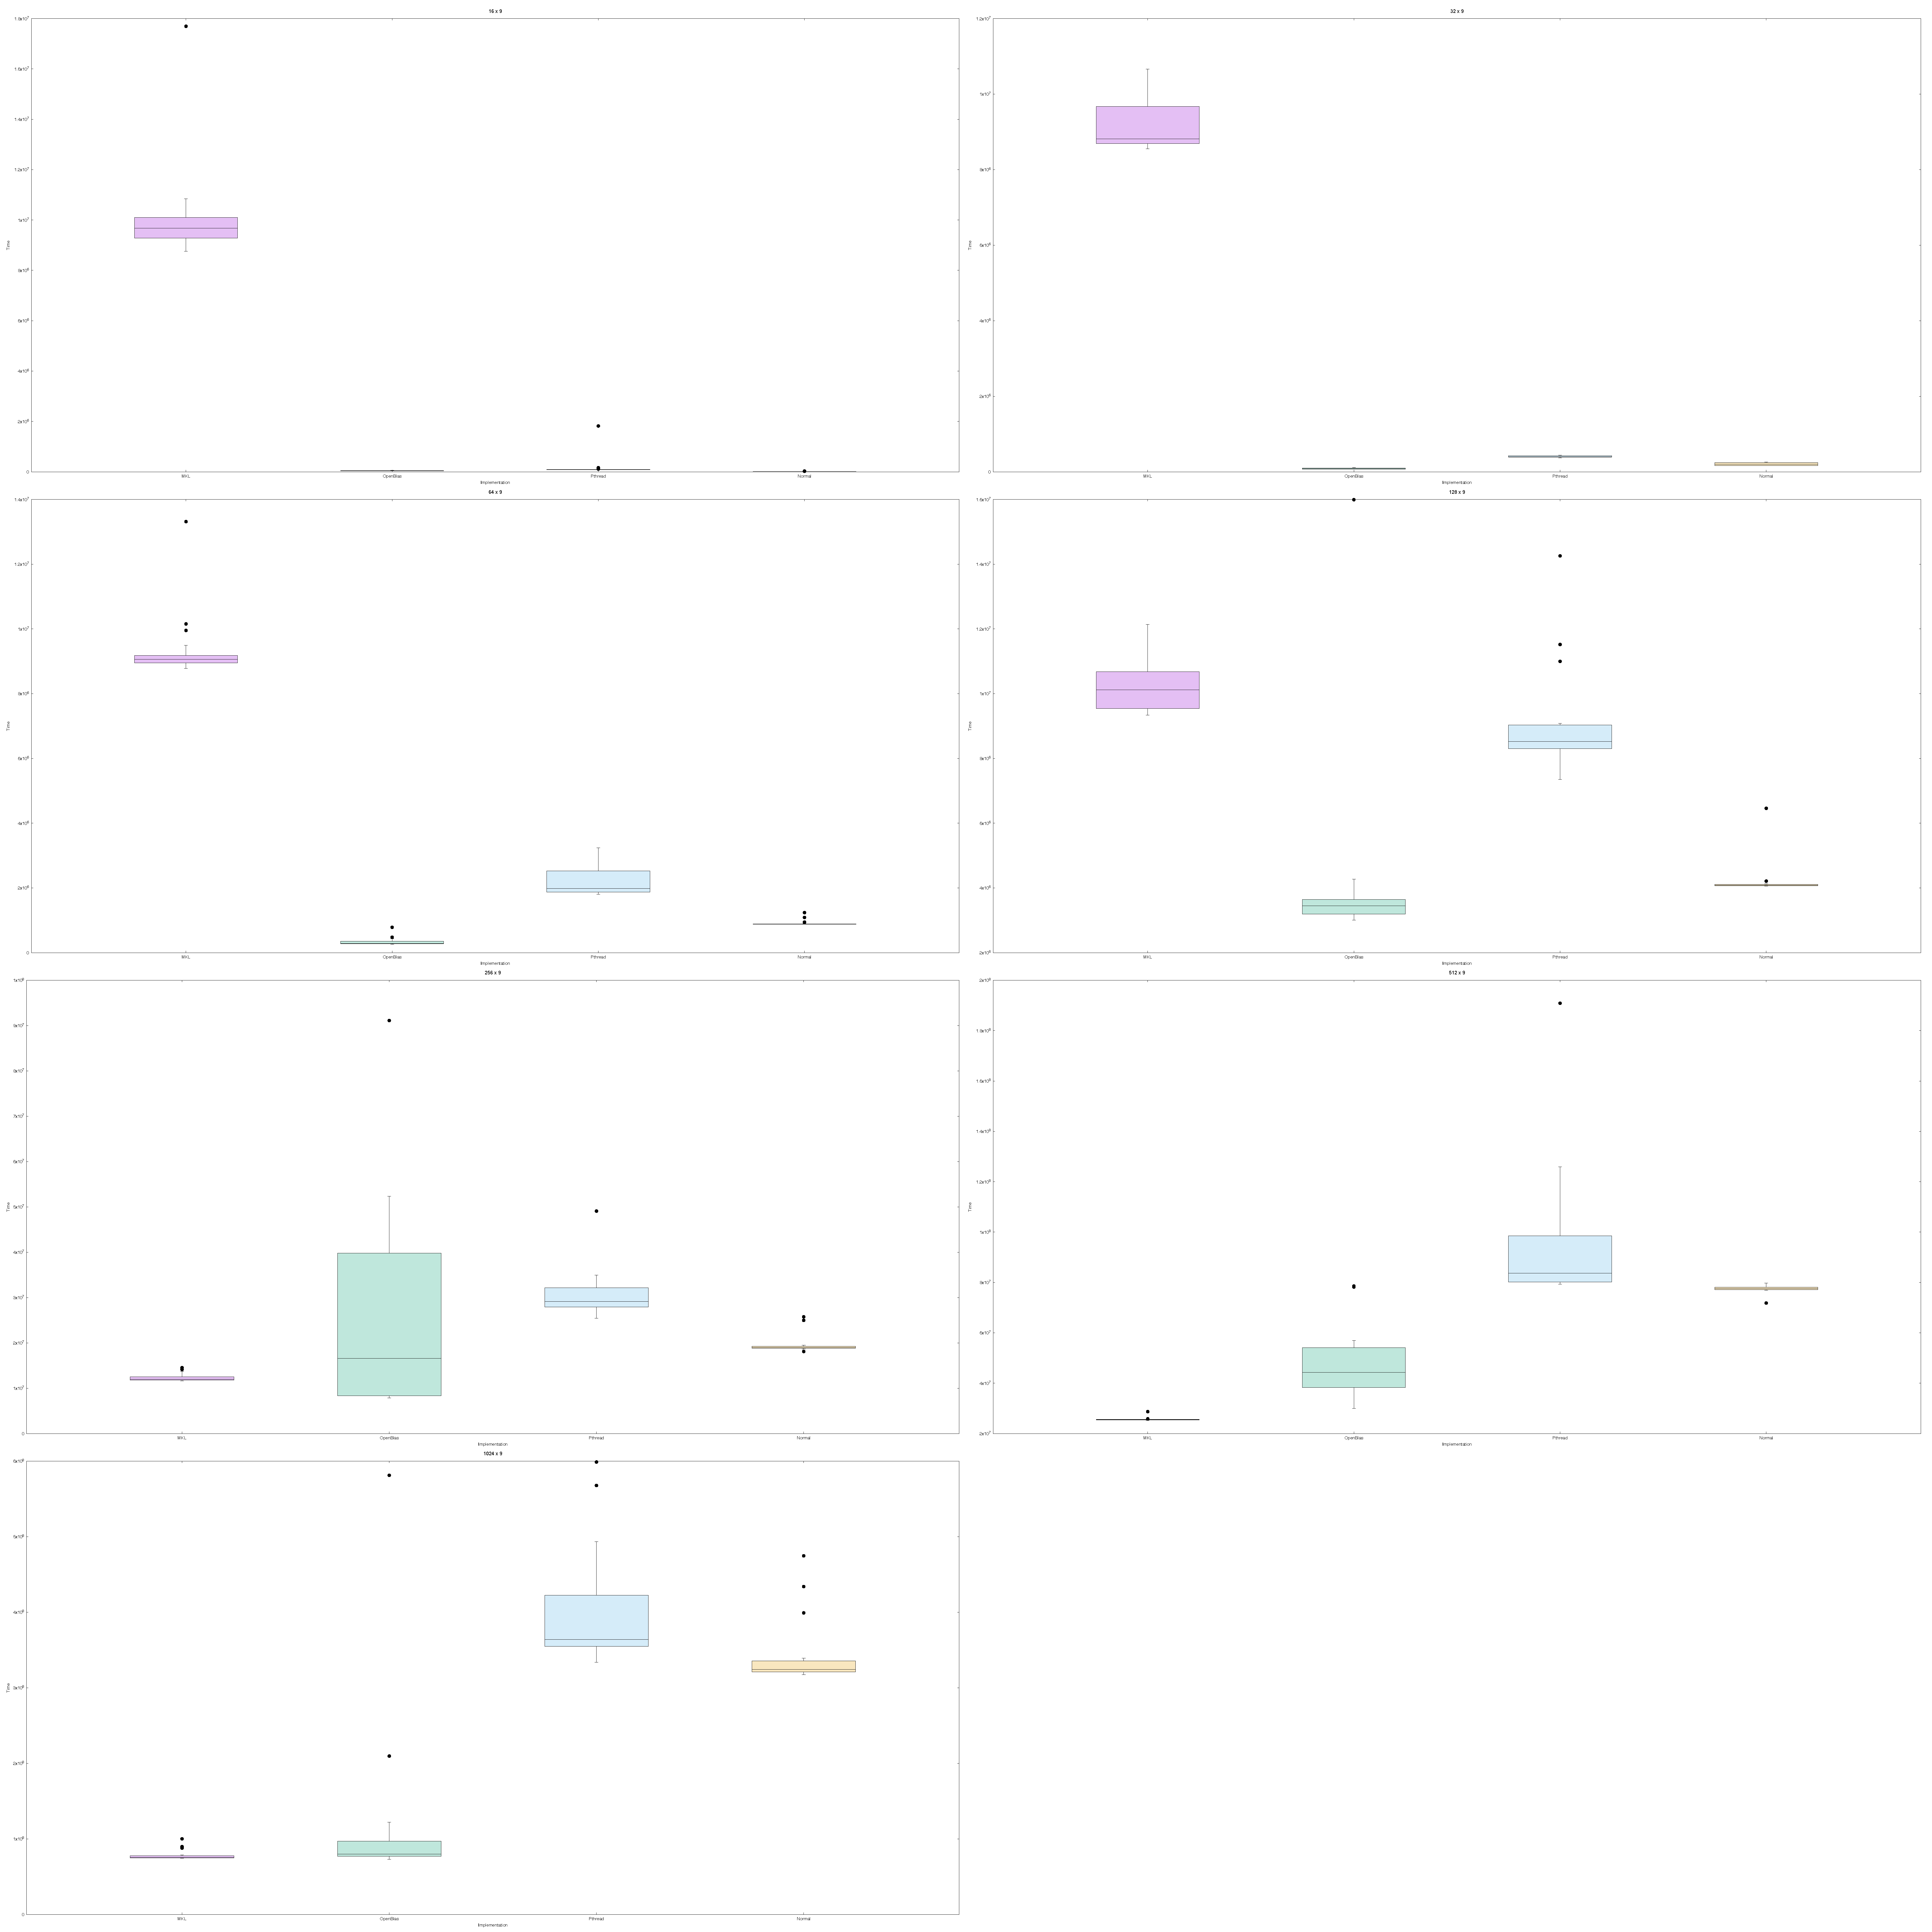
\includegraphics[width=\linewidth]{graph3.eps}


\section{Error Handling:}

\begin{itemize}
\tightlist
\item
  In case of incorrect function argument, it displays the valid function
  arguments which can be given.
\item
  In case of incorrect number of arguments, it displays the whole input
  format for the respective function.
\item
  Compulsion on the number of rows and columns(or the length of vector)
  to be always positive.
\item
  In case of convolution, error message is printed if the kernel size is
  larger than the size of the input matrix.
\item
  In case of invalid file input or invalid data type input for size of
  arrays, an exception is thrown.
\end{itemize}


\cite{MKL}.\\
\cite{OpenBLAS}.

\bibliographystyle{plain}
\bibliography{References.bib}
\end{document}






